\cotefile{156-7}
\scanpage{80}
\mspage{79}
% slanted
\margin{En dehors des cas \unsure{quasi-ensembliste|quasi-ensemblistes} et \unsure{ensembliste|ensemblistes} ces questions n'ont d'intérêt que pour des $A_i$ formés d'éléments mutuellement compatibles - - - -}

Qu'en est-il des formules pour les Sup et les Inf ? Moyennant passage aux complémentaires, on est réduit à celle sur les Inf, qui est l'inclusion
\[
\deleted{\unsure{\subset}}\quad |\bigcap A_i|\mathrel{\overset{\text{?}}{\overset{=}{\subset}}}\bigcap_i|A_i| \tag*{(X)}
\]
(les $A_i$ des parties-supports). \deleted{\unsure{Prenons} le complément des premiers, soit $\deleted{\unsure{U}}U$ il \deleted{\unsure{faut}} \deleted{\unsure{donc}} \unsure{montrer}}
\[
\deleted{U\cap\bigcap_i|A_i|=\varnothing\quad\text{??}}
\]
\deleted{Or par Hyp,}
\[
\deleted{U=|\bigvee_i\unsure{A'_i|A_i}|}
\]

Je ne sais pas aller plus loin, sauf si je fais l'hypothèse draconienne suivante, beaucoup plus forte que la précédente :
\[
\text{\uline{Hyp'}}\quad \forall a\in\unsure{\mathbb{R}|\mathbb{P}|P},\quad\exists X\in M\text{ avec }|X|=\{a\}.
\]
Ceci implique déjà la séparation $(\unsure{\mathrm{vi}'|\mathrm{vi}|\mathrm{v}'}_{\unsure{M|\mu}}\,1\mathrm{b}\unsure{,|)})$, la compatibilité de $\overline{\Sigma}_M\mathrel{\unsure{-|\longrightarrow}}\unsure{\mathcal{P}|\mathscr{P}}(P)$ aux applications $\mathrm{C}$ (plus gén. la formule
\[
|\operatorname{cosupp}A|=P\smallsetminus|A|\qquad\forall A\subset M,
\]
) je dis que ça implique aussi \uline{l'égalité dans} (X) ci dessus. Soit en effet un pt $a$ du second membre, \deleted{$\unsure{\forall_i}$}, soit $X\in M$ \inserted{\unsure{lui-même|équivalent}} avec $|X|=\{a\}$, on a \deleted{\unsure{donc} $\forall$} $|X|\subset|A_i|$ \deleted{$\unsure{\Rightarrow}$} $\operatorname{supp}X\subset\underset{\inserted{\unsure{=A_i|A_i}}}{\operatorname{supp}A_i}$

\scanpage{81}
\mspage{80}
i.e $X\in A_i$, donc $X\in\bigcap A_i$, donc $|X|\subset|\bigcap A_i|$ d'où $a\in|\bigcap A_i|$.

On trouve ainsi

\uline{Proposition} Soit $M$ un \unsure{Antos|Autos}, \deleted{\unsure{et de}} $P$ un ens, et
\[
X\longmapsto|X|:\quad M\longrightarrow\unsure{\mathcal{P}|\mathscr{P}}(P)
\]
satisfaisant les conditions suivantes :
\[
\text{\uline{\unsure{Supp}}}_{P}^{1}\quad
\deleted{\unsure{P=\bigcup_{X\in M}|X|}}\quad
\forall X,Y\in M,\qquad X\mathrel{\Vert}Y\Longleftrightarrow|X|\cap|Y|=\varnothing
\]
\[
\text{\uline{Supp}}_{P}^{2}\quad
\forall x\in\unsure{\mathbb{R}|\mathbb{P}|P},\quad\exists X\in\unsure{M|\mathbb{M}}\text{ t.q. }|X|=\{x\}
\]
Posons, pour tout $A\in M$,
\[
|A|\overset{\text{def}}{=}\bigcup_{X\in A}|X|.
\]
\uline{Alors} on a ce qui suit

(i) $\forall A\subset M$, on a
\[
|A|=\operatorname{supp}A
\]
\deleted{(ii) \unsure{Po}}
\[
|\operatorname{cosupp}A|=P\smallsetminus|A|.
\]
(\deleted{\unsure{iii}}ii) Pour $A,B\subset M$, on a
\[
\begin{aligned}
1^{\circ})\quad&\operatorname{supp}A\subset\operatorname{supp}B\quad\Longleftrightarrow\quad|A|\subset|B|\\
&\text{i.e }A\subset\operatorname{supp}B\\[3pt]
2^{\circ})\quad&A\mathrel{\Vert}B\quad\Longleftrightarrow\quad|A|\cap|B|=\varnothing
\end{aligned}
\]
\margin{Ceci est valable sans $\mathrm{Supp}^{2}$ \unsure{et aussi pour|et vrai pour} \unsure{réunions}. $\nearrow$}

(\deleted{\unsure{iv}}iii) L'application
\diagram{\begin{tikzcd}[ampersand replacement=\&,column sep=large]
\Sigma_{\unsure{M|\mu}} \arrow[r,shift left=1ex] \arrow[r,shift right=1ex,"\sim"'] \& \mathcal{P}(P) \& A \arrow[r,mapsto] \& |A|
\end{tikzcd}}
est \deleted{bijective,} un iso. d'ens. ordonnés commutant aux op. $\mathrm{C}$.

\scanpage{82}
\mspage{81}
\uline{NB} Ceci détermine $P$ et l'application $A\longrightarrow|A|$ à iso can près.
\margin{Je présume que les conditions $(\mathrm{i}_{\unsure{M|\mu}})$ $(\unsure{\mathrm{ii}'_M|\mathrm{iii}'_M|\mathrm{iii}_M})$ $(\mathrm{iv}_M)$, $(\mathrm{v}_M)$ (ou $\mathrm{At\ L\,2}$) seront satisfaites automatiquement...}

Je pense notamment, en dehors du cas des \unsure{Antos|Autos} quasi-ensemblistes, au cas où on part d'un espace topologique $P$, et où on définit $\unsure{L|\mathcal{L}}$ \inserted{(``lieux'')} comme l'ens des parties compactes contractiles \inserted{de $P$} disons.

\margin{$\unsure{\uparrow|1}$}
On construit des ``quasi-simplexes'' de tte dimension \inserted{\unsure{arbitraire}} (ou de dimension \unsure{comb.|cohom.} majorée, p. ex. par $1$) par des conditions ad hoc, généralisant celles qui définissent une \unsure{fameuse} ficelle. [Dans le cas de $\dim\leq1$, j'ai \unsure{eu|bien} une définition en forme \unsure{ds|dans} l'esprit]. On définit $|X|$ de façon évidente. Tout marche ! Mais on fera attention que si on se borne aux lieux qui se trouvent sur une ficelle donnée, et à la fonction support ci dessus, la condition $\mathrm{Supp}_P^2$ n'est plus satisfaite en général.

% slanted
\margin{Attention, ici la fonction $X\longmapsto|X|$ ne satisfait pas $\mathrm{Supp}_P^1$.}
\uline{Exemple} Je prends la ``ficelle à deux brins''
\figure{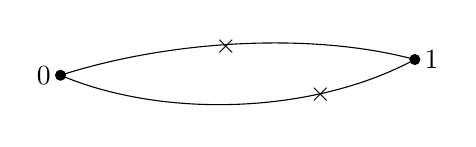
\begin{tikzpicture}[x=1cm,y=1cm]
\draw (0,0) .. controls (1.4,.45) and (3.2,.55) .. (4.5,.2);
\draw (0,0) .. controls (1.3,-.55) and (3.2,-.5) .. (4.5,.2);
\fill (0,0) circle (2pt) node[left] {$0$};
\fill (4.5,.2) circle (2pt) node[right] {$1$};
\node at (2.1,.37) {$\times$};
\node at (3.3,-.24) {$\times$};
\end{tikzpicture}}
dont les lieux \inserted{(en dehors de $0,1$)} \unsure{seront les|sont les} ``sections'' \inserted{\unsure{fermées}} de l'un et l'autre brin -- ils s'identifient donc \deleted{aux} aux éléments de l'ens ordonné produit
\[
I^{\circ}=\mathopen{]}0,1\mathclose{[}\times\mathopen{]}0,1\mathclose{[}.
\]

\scanpage{83}
\mspage{82}
Plus généralement, on peut prendre deux ensembles ordonnés $I,I'$, \deleted{Prendre le} \inserted{sans extrémités} (totalement si on veut) prendre le produit $I\times I'$, et rajouter un plus petit et un plus grand élément (``origine'' et ``extrémité''), \unsure{ceci pour former} $J$
\[
z=(x,x')\in J^{\circ}=I\times I'
\]
on voit que
\[
A_z=\{z\}
\]
est un \unsure{ensemble} support, car \unsure{ce sera} le cosupport de l'ens des \deleted{\unsure{parties}} \inserted{\unsure{Antos|Autos}} de la forme
\[
\deleted{\unsure{J_{\geq z'}}}\qquad
\begin{aligned}
[z'',1]&\quad\text{pour }z''>z\\
[0,z']&\quad\text{pour }z'<z
\end{aligned}
\]
Considérons la fonction-support \deleted{qui \unsure{prend}} \inserted{naturelle} à valeurs dans $I\amalg I'\amalg\{0\}\amalg\{1\}$
\[
\begin{aligned}
|z|&=\{x,x'\}\qquad\text{si }z=\unsure{\{x,x'\}|(x,x')}\quad x\in I,\\
|\deleted{\unsure{z}}0|&=\{0\}\\
|1|&=\{1\}
\end{aligned}
\]
Le cosupport de $A_z$ est
\[
B_z=\{z'\in J\mid z'<z\text{ ou }z'>\deleted{\unsure{J}}z\}
\]
\uline{Et on} voit tout de suite que
\[
\deleted{\unsure{B_{z_1}\cap B_{z_2}=}}\qquad
|B_z|=J\smallsetminus|z|\qquad\text{comme il se doit}
\]
Mais si $z_1,\unsure{z_2^{+}|z_2^{*}|z_2}$ ne sont pas \unsure{incomparables|comparables|incompatibles}, on aura
\[
|B_{z_1}\cap B_{z_2}|\subsetneq|B_{z_1}|\cap|B_{z_2}|
\]
\figure{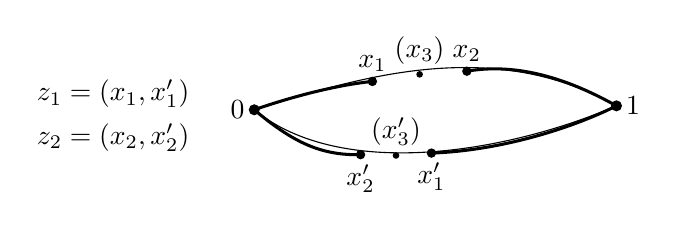
\begin{tikzpicture}[x=1cm,y=1cm]
\draw (0,0) .. controls (1.3,.4) and (3,.95) .. (4.6,.05);
\draw (0,0) .. controls (1.1,-.9) and (3.2,-.55) .. (4.6,.05);
\draw[line width=1.1pt] (0,0) .. controls (.4,.14) and (1,.31) .. (1.5,.36);
\draw[line width=1.1pt] (2.7,.49) .. controls (3.45,.62) and (4.15,.3) .. (4.6,.05);
\draw[line width=1.1pt] (0,0) .. controls (.5,-.42) and (.85,-.58) .. (1.35,-.57);
\draw[line width=1.1pt] (2.25,-.55) .. controls (3.1,-.52) and (4,-.25) .. (4.6,.05);
\fill (0,0) circle (2pt) node[left] {$0$};
\fill (4.6,.05) circle (2pt) node[right] {$1$};
\fill (1.5,.36) circle (1.7pt) node[above] {$x_1$};
\fill (2.1,.45) circle (1.2pt) node[above] {$(x_3)$};
\fill (2.7,.49) circle (1.7pt) node[above] {$x_2$};
\fill (1.35,-.57) circle (1.7pt) node[below] {$x'_2$};
\fill (1.8,-.58) circle (1.2pt) node[above] {$(x'_3)$};
\fill (2.25,-.55) circle (1.7pt) node[below] {$x'_1$};
\node[anchor=east] at (-.7,.2) {$z_1=(x_1,x'_1)$};
\node[anchor=east] at (-.7,-.35) {$z_2=(x_2,x'_2)$};
\end{tikzpicture}}
Il manque $\mathopen{]}\unsure{z_1|x_1},\unsure{z_2|x_2}\mathclose{[}$ sur $I$ et $\mathopen{]}\unsure{z'_2|x'_2},\unsure{z'_1|x'_1}\mathclose{[}$ sur $I'$

ou dualement
\[
[x_1,x_2]\cup[x'_2,x'_1]=|A_{z_1}\vee A_{z_2}|\supsetneq|A_{z_1}|\cup|A_{z_2}|=\{x_1,x_2,x'_1,x'_2\}
\]

\scanpage{84}
\mspage{83}
Soit d'autre part
\[
A=\{z_1,z_2\}
\]
on aura donc
\[
|A|=|z_1|\cup|z_2|=\{x_1,x_2,x'_1,x'_2\unsure{)|\}}
\]
mais $\operatorname{supp}A=A_{z_1}\vee A_{z_2}$ donc
\[
|\operatorname{supp}A|=[x_1,x_2]\unsure{\vee|\cup}[x'_1,x'_2]
\]
\unsure{il y a} donc
\[
|A|\subsetneq|\operatorname{supp}A|.
\]
Considérons \unsure{le} $z_3=(x_3,x'_3)$ avec
\[
\begin{aligned}
x_1<x_3<x_2,\\
x'_2<x'_3<x'_1
\end{aligned}
\]
et
\[
\begin{aligned}
A_{z_3}\cap(A_{z_1}\vee A_{z_2})&=A_{z_3}\\
(\underbrace{A_{z_3}\cap A_{z_1}}_{\varnothing})\vee(\underbrace{A_{z_3}\cap A_{z_2}}_{\varnothing})&=\varnothing
\end{aligned}
\]
donc on n'a pas la propriété modulaire de distributivité de $\cap$ p.r. à $\vee$ !

\uline{Conclusion}-\uline{Scholie} Le formalisme des supports est bon, \deleted{(en dehors des cas} pourvu qu'on ne s'avise pas de comparer les supports des strates et des figures \deleted{\unsure{pas, qui ne soient}} \inserted{qui ne soient} compatibles, ou qui ne puissent l'être moyennant subdivision. (Tel est le cas des \unsure{miens|miens,} en dehors de la situation quasi-ensembliste, ou \unsure{plus génl.|plus général.}, la situation formelle dégagée page $80$.)
% Double vertical emphasis strokes alongside the conclusion.
\margin{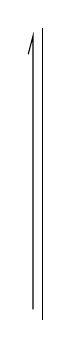
\begin{tikzpicture}\draw (0,.03)--(0,3.5)--(-.06,3.27);\draw (.12,-.1)--(.12,3.6);\end{tikzpicture}}

\scanpage{85}
\mspage{84}
C'est cette intuition que je voudrais maintenant essayer de cerner de plus près.

\figure{\begin{tikzpicture}\draw (0,.5)--(.25,0);\end{tikzpicture}}

Soit $\unsure{\mathscr{F}|\mathscr{E}}$ un atlas, $F$ une figure, $\widetilde F=I$ l'ens ordonné de ses strates.

\deleted{Dans le cas où $\operatorname{supp}_{\mathscr{F}}F=\unsure{J|I}$}

Intuitivement, on va identifier les éléments de $I$ à des ``strates ouvertes'', et on veut identifier $\unsure{\mathcal{P}|\mathscr{P}}(I)$ à \deleted{quelque} un ensemble de supports (réunions de ``strates ouvertes'').

Soit $X$ une strate. On a envie de donner un sens intrinsèque à ``$X\smallsetminus\unsure{\partial|\delta}X$'', L'idée est de \deleted{prendre} définir
\[
X^{\circ}=\operatorname{supp}_{\unsure{M|\mu}}X\cap\operatorname{cosupp}_M\partial X\qquad(\subset M)
\]
où je rappelle
\[
\partial X=\{Y\in M\mid Y\leftarrow X\}=\widetilde X\smallsetminus\{X\}
\]
On aimerait déjà vérifier que
\[
\operatorname{supp}X=\underset{Y\in X}{\operatorname{Sup}}\,Y^{\circ}
\]
\margin{Sup dans $\overline{\Sigma}_M$}
i.e, passant aux supports complémentaires
\[
\operatorname{cosupp}X=\bigcap_{Y\in\widetilde X}\deleted{\operatorname{cosupp}}\unsure{\mathbb{C}_M|\mathrm{C}_M}(Y^{\circ})
\]

\scanpage{86}
\mspage{85}
i.e. $\forall Z\in\unsure{M|\mu}$
\[
Z\mathrel{\Vert}X\Longleftrightarrow\forall Y\in\widetilde X,\quad Z\mathrel{\Vert}Y^{\circ}
\]
Bien sûr, comme $Y^{\circ}\subset\operatorname{supp}Y\subset\operatorname{supp}X$ et $Z\mathrel{\Vert}X\Leftrightarrow Z\mathrel{\Vert}\operatorname{supp}X$, l'implication $\Longrightarrow$ est claire. Donc il s'agit de voir si l'inverse est vrai. \deleted{Il faudrait donc analyser la condition}
\[
Z\mathrel{\Vert}Y^{\circ}
\]
\deleted{Je proposerai le critère heuristique provisoire}

\deleted{\uline{Critère}}
\[
\deleted{Z\mathrel{\Vert}Y^{\circ}\Longleftrightarrow\exists\text{ subdivision}\,\unsure{\circ|.}}
\]
\deleted{$Z'$ de $Z$, et une sous-figure $Z'_0$ de $Z'$, telle que}
\[
\deleted{Z'_0\ll\unsure{\partial|\delta}Y}
\]
\deleted{et}
\[
\deleted{\text{``}Z'\smallsetminus Z'_0\text{''}\mathrel{\Vert}Y}
\]

Je voudrais comparer $\unsure{X^{b}|X^{\flat}|X^{\circ}}$ et $\operatorname{supp}\operatorname{amb}(X)^{\circ}$. Je dis que
\[
\operatorname{supp}\operatorname{amb}(X)^{\circ}\subset X^{\circ}\tag*{(\alpha).}
\]
Ce qui revient (puisqu'on sait \inserted{$\mathrm{At\ L\,2}$} qu'\deleted{il} \inserted{le premier} est contenu dans $\operatorname{supp}(\operatorname{amb}(X))=\operatorname{supp}X$\unsure{,|)} à voir que $\operatorname{supp}$ est contenu dans $\operatorname{cosupp}\partial X$, i.e. \deleted{\unsure{amb}} $\operatorname{amb}(X)^{\circ}\mathrel{\unsure{\Vert|\nparallel}}\deleted{\unsure{\in|\subset}}\partial X$, ce qui \deleted{\illegible{1}} \inserted{\unsure{Compte tenu|(Compte tenu}} \deleted{$\mathrm{At\ L\,2}$} \unsure{de|en} $\mathrm{At\ L\,2}$) est $\mathrm{At\ L\,3}$. \deleted{\unsure{A-t-|A-t-on}} A-t-on égalité ?
